\section{Applications and Evaluation}

We evaluate our formalization and implementation of the SFT product operation in two key application domains: string sanitization and string replacement operations in string solving. These applications demonstrate the practical utility of our certified SFT product operation in real-world scenarios.
\subsection{Sanitizer}

An important application of our formalization lies in string sanitization for web applications. Sanitizers are crucial for preventing security vulnerabilities such as cross-site scripting (XSS) attacks by ensuring that user inputs are properly encoded before rendering in web browsers. Listing \ref{lst-html-encode} presents a C\# code snippet implementing an HTML encoding function—a fundamental sanitization operation. This function iterates through each character in the input string and encodes characters that are unsafe for HTML rendering.



\begin{lstlisting}[language={[Sharp]C}, caption={C\# Code for AntiXSS.EncodeHtml version 2.0.}, label={lst-html-encode}, float=htbp]
static string EncodeHtml(string t)
{
  if (t == null) { return null; }
  if (t.Length == 0) {
    return string.Empty;
  }
  StringBuilder builder = new
    StringBuilder("", t.Length * 2);
  foreach (char c in t) {
    if ((((c > ''') && (c < '{')) |$\mid\mid$|
         ((c > '@') && (c < '['))) |$\mid\mid$|
         (((c == ' ') || ((c > '/') && (c < ':'))) |$\mid\mid$|
         (((c == '.') || (c == ',')) |$\mid\mid$|
         ((c == '-') || (c == '_'))))) {
          builder.Append(c);
      }
      else {
          builder.Append("&#" +
          ((int) c).ToString() + ";");
      }
  }
  return builder.ToString();
}
\end{lstlisting}

Figure \ref{fig:html-sanitizer-sft} illustrates the SFT representation of the HTML encoding sanitizer function. The transducer accepts any input string and produces an output where safe characters are preserved using the identity function $\texttt{id}$, while unsafe characters are encoded as HTML entities. The set of safe characters is defined as $\texttt{safe\_chars} = [\texttt{' '}, \texttt{','}, \texttt{'.'}, \texttt{'-'}, \texttt{'\_'}] \cup [\texttt{'0'}-\texttt{'9'}] \cup [\texttt{'A'}-\texttt{'Z'}] \cup [\texttt{'a'}-\texttt{'z'}]$, which can be efficiently represented using the interval algebra we formalized. Unsafe characters are transformed using the encoding function $\texttt{encode}(c) = \texttt{``\&\#''} + \texttt{toString}(\texttt{ord}(c)) + \texttt{``\;''}$. When the alphabet is set to Unicode $[\mathtt{0x0000}, \mathtt{0x10FFFF}]$, the complement $\neg\texttt{safe\_chars}$ represents all Unicode characters outside the safe set, which can also be efficiently represented using our formalized interval operations.
\begin{figure}[htbp]
\centering
\begin{tikzpicture}[shorten >=1pt, node distance=2.5cm, on grid, auto]
  % States
  \node[state, initial, accepting] (q0) {$q_0$};
  \node[state] (q1) [right=3.5cm of q0] {$q_1$};
  \node[state] (q2) [below=of q0] {$q_2$};
  
  \path[->] 
    % Transition for safe characters
    (q0) edge[bend left=20] node[above,midway=1] {$\texttt{safe\_chars}, \texttt{id}$} (q1)
    % Transition for unsafe characters  
    (q0) edge[bend right=20] node[left,midway] {$\neg\texttt{safe\_chars}, \texttt{encode}$} (q2)
    % Epsilon transitions back to q0
    (q1) edge[bend left=30] node[below,midway] {$\varepsilon, \lambda\varepsilon$} (q0)
    (q2) edge[bend right=20] node[right,midway] {$\varepsilon, \lambda\varepsilon$} (q0);
\end{tikzpicture}
\caption{SFT representation of the HTML encoding sanitizer function.}
\label{fig:html-sanitizer-sft}
\end{figure}

We evaluate the performance of our SFT product operation by computing the product of the HTML encoding sanitizer SFT with SFAs constructed from randomly generated Unicode user inputs. This experimental setup reflects realistic usage scenarios where diverse character sets and input patterns are encountered. The experimental evaluation was conducted on a laptop with an Apple M4 processor and 24 GB of memory, with a one-minute time limit per test.

Figure \ref{fig:benchmark-results} demonstrates the scalability characteristics of our SFT product implementation. The computation requires approximately 1 second for 100,000-character inputs and 10 seconds for 1,000,000-character inputs. These performance metrics confirm that our certified implementation maintains computational efficiency suitable for practical string processing applications at scale.

\begin{figure}
\centering
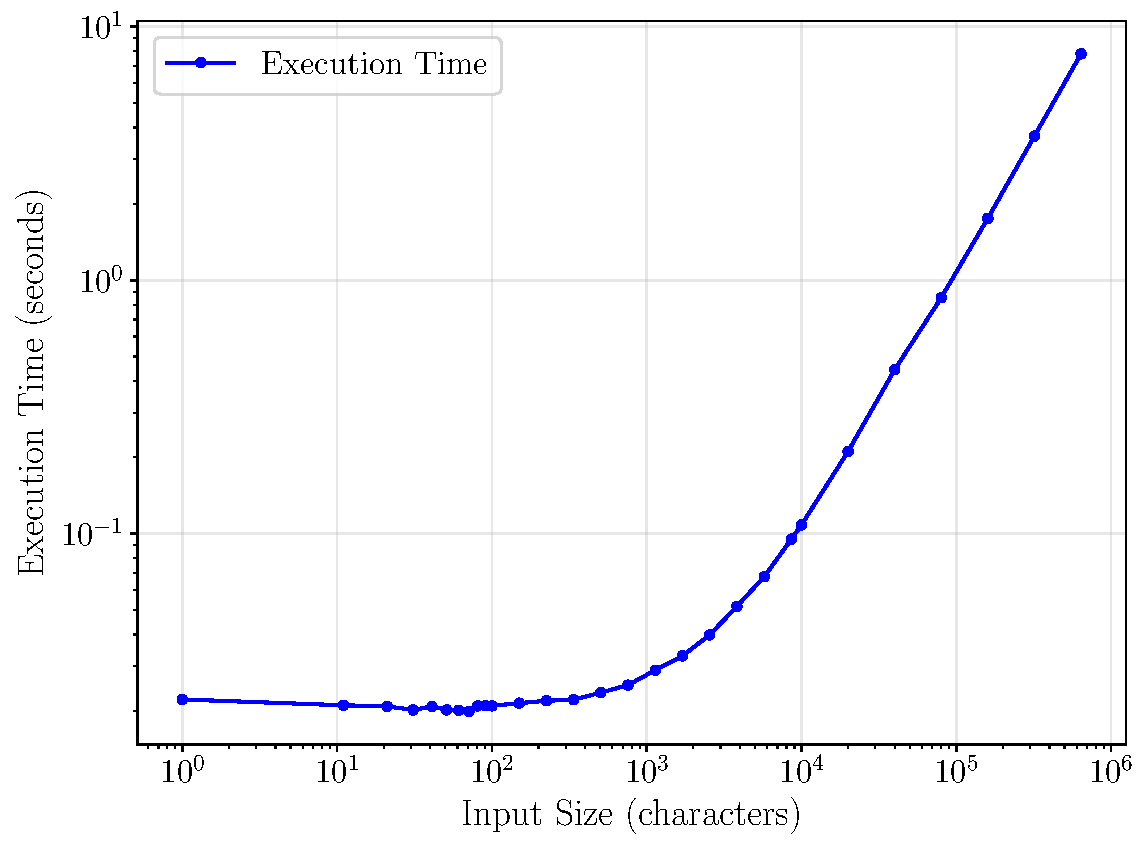
\includegraphics[scale=0.45]{benchmark_loglog.pdf}
\caption{Experimental results for the sanitizer product}
\label{fig:benchmark-results}
\end{figure}

Beyond performance evaluation, our SFT formalization enables formal verification of string sanitizer correctness. A santizer is used to transform user inputs into safe outputs, ensuring that the output does not contain any unsafe characters. However, santizers just like programs, which are eror-prone. Manual reviews of sanitizers are often insufficient to guarantee correctness.

Based on our formalization, we can verify sanitizers by modeling the sanitizer as an SFT and the user input as an SFA. We can also model potential attacks as SFAs that accept unsafe strings. Formally speaking, Let $\mathcal{T}$ be an SFT, $\mathcal{I}$ is the possible user inputs modeled by an SFA, and $\mathcal{A}$ is the attack SFA that accepts unsafe strings. The santizer correctness checking against the attack is to check whether the intersection of the product $\mathcal{T} \times \mathcal{I}$ and the attack SFA $\mathcal{A}$ is empty, i.e., $\mathcal{T} \times \mathcal{I} \cap \mathcal{A} = \emptyset$.

Moreover, santizers are usually used in combination with other sanitizers to ensure comprehensive safety. For example, the HTML encoding sanitizer can be combined with a string trimming operation to remove leading and trailing whitespace characters. For this kind of sanitizer composition, it can be modeled by our SFT product as well. Let $\mathcal{T}_1$ and $\mathcal{T}_2$ correspond to two sanitizers, and $\mathcal{T}_1$ is applied before $\mathcal{T}_2$. What we need to check is $\mathcal{T}_2 \times (\mathcal{T}_1 \times \mathcal{I}) \cap \mathcal{A} = \emptyset$.




\begin{table}[h]
  \centering
  \small
  \setlength{\tabcolsep}{4pt} % Reduced column gap
  \begin{tabular}{p{2.2cm}ll} % Increased width for automatic line break
    \toprule
    \textbf{Attack Model} & \textbf{Verfication Result} & \textbf{Size} \\
    \midrule
    attack\_html           & GA HtmlEscape: \textbf{Unsafe} & 1/6\\
                           & Trim + GA HtmlEscape: \textbf{Safe} & 4/12 \\
                           & escapeString: \textbf{Unsafe} & 1/11 \\
                           & Trim + escapeString: \textbf{Safe} & 4/17 \\
                           & Trim + OWASP HTMLEncode: \textbf{Safe} & 4/18 \\
    \midrule
    attack\_javascript     & GA Htmlescape + GA PreEscape + & 3/20 \\
                           &  gaSnippetesc: \textbf{safe} & \\
    \midrule
    attack\_json           & Trim + GA JSONESc : \textbf{Safe} & 4/16\\
    \midrule
    attack\_xml            & Trim + GA XMLEsc: \textbf{safe} & 4/16\\
    \midrule
    attack\_ccs            & Trim + GA CleanseCSS : \textbf{Safe} & 25/46\\
    \bottomrule
  \end{tabular}
  \caption{Sanitizer verfication result}
  \label{tab:sanitizer_attack}
\end{table}

Table \ref{tab:sanitizer_attack} summarizes the verification results for various sanitizers against different attack models. The first column lists the attack models, the second column indicates whether the sanitizer is classified as safe or unsafe with respect to the attack, and the third column reports the size of the transducers used in the verification, given as [number of states/number of transitions]. For composed SFTs, the size reflects the total number of states and transitions across all components.

We evaluate a range of attack models for HTML, JavaScript, JSON, XML, and CSS. Listing \ref{lst-css-attack} shows the CSS attack model, which is used to verify the corresponding sanitizer. The attack model includes comments, declaration breakers, and known dangerous tokens such as \textbf{expression(}, \textbf{@import}, \textbf{behavior:}, \textbf{-moz-binding}, and \textbf{url(} (unless the URL is separately validated). Sanitizers include GA HtmlEscape, GA JSONEscape, GA XMLEscape, escapeString, and GA CleanseCSS, where "GA" means from Google. Sanitizers are often composed with preprocessing steps such as Trim, which removes leading and trailing whitespace characters. As shown in the table, GAHtmlEscape and escapeString are unsafe with respect to the HTML attack model without preprocessing, but become safe when combined with Trim. The \textbf{Size} column demonstrates the expressive power and succinctness of SFTs in modeling real-world transducers.




\begin{lstlisting}[language={}, caption={CSS attack model for sanitizer verification.}, label={lst-css-attack}, float=htbp]
|$\Sigma$|* ( / \* [\s\S]*? \*/
  |$\mid$| ; |$\mid$| \{ |$\mid$| \}
  |$\mid$| [eE][xX][pP][rR][eE][sS][sS][iI]
    [oO][nN]\s*\(
  |$\mid$| @\s*[iI][mM][pP][oO][rR][tT]
  |$\mid$| [bB][eE][hH][aA][vV][iI][oO][rR]\s*:
  |$\mid$| -\s*[mM][oO][zZ]-\s*[bB][iI][nN]
    [dD][iI][nN][gG]
  |$\mid$| (?!allowUrl) [uU][rR][lL]\s*\(
 ) |$\Sigma$|*
\end{lstlisting}

\subsection{Modeling the Replacement Operation}

The string replacement operation, denoted as
$\texttt{replace}(\texttt{str}, \newline\texttt{pattern}, \texttt{replacement})$, is a fundamental string transformation that takes three parameters:
\begin{itemize}
  \item $\texttt{str}$: The input string to be transformed.
  \item $\texttt{pattern}$: A regular expression defining the matching criteria.
  \item $\texttt{replacement}$: The string to be substituted for the matched substring.
\end{itemize}

The semantics of the replacement operation can be formally characterized by two distinct cases:
\begin{enumerate}
  \item When there exists at least one substring $s'$ in \texttt{str} such that $s'$ matches $\texttt{pattern}$, then $s'$ is replaced with \texttt{replacement}.
  \item When no substring of \texttt{str} matches $\texttt{pattern}$, the operation returns \texttt{str} unchanged.
\end{enumerate}

The first case can be modeled by SFTs. We illustrate this case by an example. Given a replacement operation $\texttt{replace}\newline(s, \texttt{/[0-9]+/}, "\texttt{NUM}")$, which means replacing a occurrence of the substring that matches the regular expression $\texttt{/[0-9]+/}$ with the string "\texttt{NUM}".
We model this replacement operation by an SFT with the following 3 steps:

\begin{enumerate}
  \item First, construct an SFA that recognizes the regular expression pattern $\texttt{/[0-9]+/}$. Transform this SFA into an SFT by augmenting each transition with an output function $f = \lambda x.~\texttt{None}$ that produces the empty string. 
  \item Second, construct an SFA that accepts the replacement string "\texttt{NUM}". Since a constant string can be viewed as a specialized regular expression, we can construct its SFA representation. Convert this SFA into an SFT by adding $\varepsilon$-transitions  and appropriate output functions that emit the characters of "\texttt{NUM}" in sequence.
  \item Finally, compose the two SFTs through concatenation and augment the resulting transducer with self-loop transitions at the initial and final states. These additional transitions, labeled with $\Sigma$ (the set of all characters in the alphabet) and the identity function $\texttt{id}=\lambda x.~x$, enable the SFT to process arbitrary prefixes and suffixes of the input string while preserving the replacement behavior on matched substrings.
\end{enumerate}


\noindent\emph{Step 1.}
Figure \ref{fig-snfa-pattern} illustrates the construction of the pattern-matching component. The left side shows the SFA that recognizes the regular expression $\texttt{/[0-9]+/}$, while the right side presents its transformation into an SFT. This transformation is achieved by augmenting each transition with the output function $\texttt{f} = \lambda x.~\texttt{None}$, which consistently produces the empty string, effectively "consuming" the matched digits without generating output.





\begin{figure}[h] \centering
\begin{tikzpicture}[shorten >=1pt, node distance=1.8cm, auto]
  % Left: SFA for [0-9]+ (vertical)
  \node[state, initial] (q0)   {$q_0$}; 
  \node[state, accepting, below=of q0] (q1) {$q_1$}; 

   \path[->] 
   (q0) edge [bend left=20] node[right] {\texttt{[0-9]}} (q1)
   (q1) edge [loop below] node {\texttt{[0-9]}} (q1);

  % Right: SFT for [0-9]+ (vertical)
  \node[state, initial, right=4cm of q0] (q0') {$q_0'$}; 
  \node[state, accepting, below=of q0'] (q1') {$q_1'$}; 

   \path[->] 
   (q0') edge [bend left=20] node[right] {\texttt{[0-9]},$\texttt{f}$} (q1')
   (q1') edge [loop below] node {\texttt{[0-9]},$\texttt{f}$} (q1');
\end{tikzpicture}
\caption{Corresponding SFA and SFT for \texttt{/[0-9]+/}}
\label{fig-snfa-pattern}
\end{figure}

\noindent\emph{Step 2.}
Figure \ref{fig-snfa-replacement} depicts the automata for the replacement string "\texttt{NUM}". The left side shows the SFA that accepts this constant string, while the right side presents its SFT transformation. The transformation employs an indexed output function \texttt{g} that emits characters of the replacement string sequentially:
\[
\texttt{g} = \lambda~i~x.~\texttt{match}~i~\texttt{with}~
\begin{cases}
1 \mapsto [(78, 78)] & \text{(ASCII for 'N')} \\
2 \mapsto [(85, 85)] & \text{(ASCII for 'U')} \\
3 \mapsto [(77, 77)] & \text{(ASCII for 'M')} \\
\_ \mapsto \texttt{None}
\end{cases}
\]
This function maps transition indices to their corresponding character outputs, using ASCII codes to represent the string "\texttt{NUM}" character by character.


\begin{figure}[h] \centering
\begin{tikzpicture}[shorten >=1pt, node distance=2cm, auto]
  % SFA for "NUM" (top)
  \node[state, initial above] (q0)   {$q_0$}; 
  \node[state] (q1) [right=1cm of q0] {$q_1$}; 
  \node[state] (q2) [below=1cm of q1] {$q_2$}; 
  \node[state, accepting] (q3) [below=1cm of q0] {$q_3$}; 

  \path[->] 
  (q0) edge node {\texttt{N}} (q1)
  (q1) edge node {\texttt{U}} (q2)
  (q2) edge node {\texttt{M}} (q3);

  % SFT for "NUM" (right)
  \node[state, initial above] (q0') [right=1.5cm of q1] {$q_0'$}; 
  \node[state] (q1') [right=of q0'] {$q_1'$}; 
  \node[state] (q2') [below=1cm of q1'] {$q_2'$}; 
  \node[state, accepting] (q3') [below=1cm of q0'] {$q_3'$}; 

  \path[->] 
  (q0') edge node {\texttt{None}, \texttt{(g 1)}} (q1')
  (q1') edge node[left] {\texttt{None}, \texttt{(g 2)}} (q2')
  (q2') edge node[below] {\texttt{None}, \texttt{(g 3)}} (q3');
\end{tikzpicture}
\caption{Corresponding SFA and SFT for "\texttt{NUM}"}
\label{fig-snfa-replacement}
\end{figure}


\noindent\emph{Step 3.}
Figure \ref{fig-rearranged-automata} presents the complete SFT construction, obtained by composing the pattern-matching SFT (Fig. \ref{fig-snfa-pattern}) with the replacement-generating SFT (Fig. \ref{fig-snfa-replacement}). The composition process involves two key modifications:
\begin{enumerate}
  \item Connect the two SFTs by adding $\varepsilon$-transitions (labeled with "\texttt{None}, \texttt{f}") from each accepting state of the pattern-matching SFT to the initial state of the replacement-generating SFT
  \item Augment the resulting transducer with self-loop transitions at both ends, labeled with "$\Sigma,~\texttt{id}$", where $\Sigma$ represents the full alphabet. For the string solver, $\Sigma$ is the set of all unicode characters. These transitions enable the SFT to process arbitrary input prefixes and suffixes while preserving the matched substring for replacement
\end{enumerate}

\begin{figure}[h] \centering
  \begin{tikzpicture}[shorten >=1pt, node distance=2cm, auto]
    % Second automaton from the first figure
    \node[state, initial] (q0') {$q_0'$}; 
    \node[state] (q1') [right=of q0'] {$q_1'$}; 
  
     \path[->] 
     (q0') edge [bend left] node {\texttt{[0-9]}, $\texttt{f}$} (q1')
     (q1') edge [loop right] node {\texttt{[0-9]}, $\texttt{f}$} (q1')
     (q0') edge [loop below] node {$\Sigma$, $\texttt{id}$} (q0');
  
    % Second automaton from the second figure
    \node[state] (q0'') [below=1cm of q1'] {$q_0''$}; 
    \node[state] (q1'') [right=of q0''] {$q_1''$}; 
    \node[state, accepting] (q3'') [below=1cm of q0''] {$q_3''$}; 
    \node[state] (q2'') [right=of q3''] {$q_2''$}; 
  
    \path[->] 
    (q0'') edge node {\texttt{None}, \texttt{(g 1)}} (q1'')
    (q1'') edge [bend left=5] node[left] {\texttt{None}, \texttt{(g 2)}} (q2'')
    (q2'') edge node {\texttt{None}, \texttt{(g 3)}} (q3'')
    (q3'') edge [loop left] node {$\Sigma$, $\texttt{id}$} (q3'')
    (q1') edge [bend right=30] node {\texttt{None}, \texttt{f}} (q0'');
  \end{tikzpicture}
  \caption{The SFT for the replacement operation \\ $\texttt{replace}(s, \texttt{/[0-9]+/}, \text{``NUM''})$}
  \label{fig-rearranged-automata}
  \end{figure}


  Having constructed the SFT, we can now compute the forward image of the replacement operation. Consider the string constraint $s' = \texttt{replace}(s,~\texttt{/[0-9]+/},~\text{"}\texttt{NUM}\text{"})$, where we aim to characterize the possible values of $s'$. Let $\mathcal{T}$ denote the constructed SFT modeling the replacement operation, and let $\mathcal{A}$ be the SFA representing the domain of possible values for the input string $s$. The forward image of this replacement operation is given by the product $\mathcal{T} \times \mathcal{A}$, which precisely captures the set of all possible output strings that can be produced by applying the replacement operation to any input string accepted by $\mathcal{A}$.
  Our string solver uses this forward image to do forward propagation for further string solving.

  
  The replacement operation model described above replaces a single occurrence of any substring matching the regular expression pattern. To support different replacement semantics, 
  we model replace-all operations (which substitute all occurrences of matching substrings).

  

  The approach to modeling replace-all operations is illustrated in Figure \ref{fig:replace-all}. 



\begin{figure}[htbp]
\centering
\begin{tikzpicture}[node distance=2cm, state/.style={circle, draw, minimum size=0.8cm}]
  % First SFT rectangle
  \node[draw, rectangle, minimum width=5.2cm, minimum height=2.1cm] (sft1-box) {};
  \node[above=0.1cm of sft1-box.north] {\textbf{SFT} $\mathcal{T}_1$ (Non-matching)};
  
  % States inside first SFT
  \node[state, initial] (p0) at ([xshift=-0.8cm]sft1-box.center) {$p_0$};
  \node[state, accepting] (p1) at ([xshift=1.8cm]sft1-box.center) {$p_1$};
  \path[->] (p0) edge[above] node {\shortstack{$\neg\texttt{pattern},$ \\ $\lambda x.x$}} (p1);
  
  % Second SFT rectangle
  \node[draw, rectangle, minimum width=5.2cm, minimum height=2.1cm, below=1.5cm of sft1-box] (sft2-box) {};
  \node[below=0.1cm of sft2-box.south] {\textbf{SFT} $\mathcal{T}_2$ (Matching)};
  
  % States inside second SFT
  \node[state, initial] (s0) at ([xshift=-0.8cm]sft2-box.center) {$s_0$};
  \node[state, accepting] (s1) at ([xshift=2cm]sft2-box.center) {$s_1$};
  \path[->] (s0) edge[above] node {\shortstack{$\texttt{pattern},$ \\ $\texttt{replacement}$}} (s1);
  
  % Epsilon transition from accepting state of first SFT to initial state of second SFT
  \path[->] (p1) edge[bend right=30] node[left] {\shortstack{$\varepsilon$, $\lambda\varepsilon$}} (s0);
  
  % Epsilon transition from accepting state of second SFT to initial state of first SFT
  \path[->] (s1) edge[bend right=30] node[right] {\shortstack{$\varepsilon$, $\lambda\varepsilon$}} (p0);
  
\end{tikzpicture}
\caption{The modeling of replace all operation.}
\label{fig:replace-all}
\end{figure}



\subsection{Experiments of String Replacement Operations}

We have implemented CertiStrR, an extension of  CertiStr \cite{cpp/KanLRS22}, to support string replacement operations.
%\footnote{The implementation is available at \url{https://github.com/ShlKan/certified-str-solver}}. 
CertiStr \cite{cpp/KanLRS22} is a certified string solver that only support some basic string operations, such as concatenation, and regular constraints. 


%While the core solving algorithm maintains the certification guarantees of CertiStrR, the frontend components are implemented using established non-certified  OCaml libraries: dolmen \cite{dolmen} for SMT-LIB parsing and ocaml-re-nfa \cite{ocaml-re-nfa} for regular expression to NFA conversion.

CertiStrR implements two different pattern matching introduced above: (1) singleton matching at any position, (2) replace-all matching. The pattern can be a regular expression or a constant string, which is a special case of regular expression.

% Listing \ref{lst-smtlib-code} demonstrates the regular expression variant through an example that replaces numeric sequences with the string "\texttt{NUM}". The constraints are satisfiable because the input string \texttt{a} = "\texttt{2024,2025}" contains a substring "\texttt{2025}" that matches the regular expression \texttt{re.+ (re.range "0" "9")} (equivalent to \texttt{/[0-9]+/}), and replacing this match with "\texttt{NUM}" yields the expected output string \texttt{b} = "\texttt{2024,NUM}".
% %
%
%
% \begin{lstlisting}[language=SMTLIB, caption={Example SMT-LIB Code}, label={lst-smtlib-code}, float=htbp]
%   (set-logic QF_S)
%   (declare-fun a () String)
%   (declare-fun b () String)
%   (assert (= a "2024,2025"))
%   (assert (= b "2024,NUM"))
%   (assert (= b (str.replace_re a 
%       (re.+ (re.range "0" "9")) "NUM")))
%   (check-sat)
%   \end{lstlisting}


We evaluate CertiStrR using benchmarks from SMT-LIB 2024 \cite{smtlib_benchmarks}, focusing on the QF\_S and QF\_SLIA logic fragments. The benchmarks are categorized into three groups based on their pattern matching semantics: (1) general singleton matching and (2) replace-all matching. Patterns can be either regular expressions or constant strings.

Due to CertiStrR's current frontend limitations in supporting the complete SMT-LIB language specification, we preprocess certain operations. For example, conjunctive assertions of the form \texttt{(assert (and c1 c2))} are decomposed into separate assertions \texttt{(assert c1)} and \texttt{(assert c2)} when both \texttt{c1} and \texttt{c2} are string constraints supported by CertiStrR.

% replace_re
% Average real time: 0.37 seconds
% Total number of real entries: 98
% Average user time: 0.35 seconds
% Total number of user entries: 98
% Average sys time: 0.01 seconds
% Total number of sys entries: 98
% Total number of SAT entries: 61
% Total number of UNSAT entries: 4
% Total number of inconclusive entries: 30

% replace_str
% Average real time: 0.27 seconds
% Total number of real entries: 323
% Average user time: 0.25 seconds
% Total number of user entries: 323
% Average sys time: 0.01 seconds
% Total number of sys entries: 323
% Total number of SAT entries: 315
% Total number of UNSAT entries: 173
% Total number of inconclusive entries: 8


\begin{table}[h]
  \centering
  \small
  \begin{tabular}{lcccc}
      \toprule
      & \textbf{SAT/UNSAT/Inc} & \textbf{Time (s)} & \textbf{Tests} \\
      \midrule
      \texttt{replace singleton} & 142/173/8 & 0.27 & 323\\
      \texttt{replace all} & 84/4/10 & 0.36 & 98\\
      \bottomrule
  \end{tabular}
  \caption{Experimental results}
  \label{tab:string_operations}
\end{table}

The experimental evaluation was conducted on a laptop with an Apple M4 processor and 24 GB of memory, with a one-minute time limit per test. The results show average execution times of 0.27 seconds for \texttt{replace singleton} and 0.36 seconds for \texttt{replace all}. Test outcomes were classified into three categories: SAT (satisfiable), UNSAT (unsatisfiable), and Inconclusive.

An "Inconclusive" result indicates that the solver cannot determine satisfiability, not due to timeout (all tests completed within one minute), but due to the inherent incompleteness of the string solver's algorithm. An inconclusive result can occur when the solver cannot decide whether a string variable can be assigned a unique value to make the constraints satisfiable.


Our performance analysis revealed that while the SFT-based replacement operation modeling is efficient, the primary computational bottleneck stems from automata accumulation during  forward-propagation. Consider the following string constraints:
\begin{align}
x &= x_1\texttt{++}x_2;~x = \texttt{replace}(x_3, p, r); \nonumber ~x = \texttt{replace\_re}(x_5, p_1, r_1); \nonumber
\end{align}
where \texttt{++} denotes string concatenation. The variable $x$ appears multiple times on the left-hand side of the equations, causing the forward-propagation algorithm to accumulate automata representations for all constraints: $x_1\texttt{++}x_2$, \texttt{replace}\newline($x_3, p, r$), $x_4$, and \texttt{replace\_re}($x_5, p_1, r_1$). Each accumulation step requires computing the product of the current automaton with the previous result. Given that the product operation has a worst-case complexity of $O(n^2)$, where $n$ represents the automaton size, this repeated accumulation can lead to state explosion.


\subsection{Effort of Certified Development}

This subsection discusses the development effort required for our certified SFT formalization. Table \ref{tab:abstract_impl} provides an overview of this effort.
Note that, to model replacement operation, we not only need the formalization of SFTs but also the formalization of negation of an SFA, $\epsilon$NFA.

All efforts listed in the table are additional to the existing CertiStr framework that we build upon.

The abstract-level development encompasses all formalizations presented in Sections \ref{sec:formalization} and \ref{sec:product-operation}, including SFTs and $\varepsilon$SFAs. The implementation-level development covers all formalizations in Section \ref{sec_alg_refinement}, including the refinement of the product operation. The final row corresponds to the interval formalization effort. The most challenging component proved to be the correctness proof of the product operation at the abstract level (Figure \ref{fig-def-product-correct}).

The interval formalization complexity increased dramatically in CertiStrR compared to the interval formalization in CertiStr \cite{cpp/KanLRS22}, primarily due to extending intervals from single pairs to lists.

\begin{table}[h]
  \centering
  \small
  \begin{tabular}{lccc}
      \toprule
      & \textbf{Defs} & \textbf{Lemmas} & \textbf{Proofs (LOC)} \\
      \midrule
      Abstract & 17 & 21 & 3274 \\
      Implementation & 51 & 43 & 2700 \\
      Interval & 15 & 29 & 1500 \\
      \bottomrule
  \end{tabular}
  \caption{Overview of the effort of certified development}
  \label{tab:abstract_impl}
\end{table}